\chapter{Implementazione}

\section{Introduzione}

Ci sono vari modi per permettere all'utente di utilizzare dei servizi tramite una applicazione. Principalmente si può sviluppare o sotto forma di app nativa o nella forma di "sito web".\\ 

\noindent
Le app native sono quelle app sviluppate appositamente per un certo sistema operativo, e i principali mobile sono Android e IOS. Per Android i linguaggi utilizzabili sono Java, C++ o il più recente Kotlin, per quanto riguarda IOS si utilizza Swift. Questi linguaggi implementano delle strutture e delle funzioni che comunicano (più o meno direttamente) con il sistema operativo del device e ne sono strettamente legati poichè mentre la logica generale dell'app può essere la stessa, certe versioni del sistema operativo o device diversi (specialmente in Android che è il sistema operativo di smartphone molto diversi tra di loro) richiedono funzioni o implementazioni di strutture diverse per comunicare con il sistema operativo\\ 

\noindent
Per quanto riguarda i "siti web", ovvero le applicazioni web gli strumenti utilizzabili sono svariati, anche perchè una applicazione web è composta da più elementi, principalmente un frontend e un backend.\\
Il frontend è ciò che "gira" su un browser e ne è dipendente, poichè il browser recupera da un server i dati dell'applicazione e li interpreta rendendoli utilizzabili dall'utente. Per quanto riguarda il frontend le tecnologie utilizzate sono html, che fornisce lo scheletro dei vari oggetti, javascript, che descrive il comportamento degli oggetti e manipola lo scheletro html, e css, che descrive lo stile degli oggetti (quindi, semplificando, posizionamento e colori).\\
Il backend è ciò che "gira" sul server. I servizi di backend sono delle API raggiungibili tramite internet a un certo indirizzo ip, in cui vi è una macchina che hosta un server che prende le richieste, inviate da un'app web o in qualsiasi altro modo, e le traduce e consegna all'applicazione richiesta, che le elabora e, eventualmente, ritorna una risposta a chi ha inoltrato la richiesta. L'utilizzo di un backend è molto utile poichè rende disponibile la potenza di calcolo di una macchina. Ad esempio nel mio caso ho bisogno di eseguire dei calcoli complessi, che sarebbero troppo pesanti da far eseguire al browser, il backend mi permette di inviare una richiesta con i dati necessari, far eseguire il calcolo e successivamente farmi ritornare il risultato. Altro utilizzo fondamentale è la comunicazione con un database, il backend può implementare la comunicazione con un database remoto o locale, il vantaggio è che l'utente si connette al backend e non al database, con moltissimi vantaggi per quanto riguarda la sicurezza.\\
Ci sono moltissimi linguaggi utilizzabili come backend, a parte i linguaggi tipo php, che necessitano solo che il file che deve eseguire le operazioni venga richiamato passando i parametri necessari, basta che abbiano modo (tramite framework o librerie) di implementare un server che si metta in ascolto su una porta che accetti le richieste e richiami le funzioni necessarie al funzionamento, eventualmente rispondendo con ciò che è stato richiesto. Generalmente (nel mio caso ad esempio) questo server in ascolto viene poi reso disponibile sul web grazie a un server web (tipo apache o nginx) che fa da proxy. Nel mio caso infatti il client comunica con il server web in ascolto sulla porta 80 comunicando un percorso (detto path) che il server web elabora rigirando la richiesta al servizio corretto.\\

\noindent
Entrambe le soluzioni presentano svantaggi e vantaggi. Le app native sono molto buone e affidabili, ma richiedono un grande lavoro di adattamento per i vari sistemi operativi e le varie versioni, banalmente bisogna sviluppare una versione Android e una IOS. Le applicazioni web invece eliminano il problema di dover adattare il codice al sistema, però possono funzionare solo tramite browser e non possono interagire con il sistema, ad esempio non possono mandare notifiche.\\
Perciò la scelta implementativa che ho adottato è lo sviluppo di una PWA.

\vspace{1cm}
\section{Cos’è una PWA}

La sigla “PWA” significa Progressive Web App, e unisce il Web alle App native. Le PWAs sfruttano le moderne capacità Web per fornire una user experience "app-like", ovvero sono come dei siti web con interfaccia e utilizzo simile a una app nativa. Ci sono però alcune differenze molto importanti con i tradizionali siti web, queste differenze sono quelle che rendono l’applicazione web simile a un’app nativa, infatti avremmo bisogno di due componenti fondamentali: il Manifest.json e un ServiceWorker.js.\\
Nel Manifest.json si  inseriscono una serie di dati utili al download e al versioning: si va a inserire la versione del manifest, la versione dell’app, il nome e le varie icone dell’app che compariranno sul nostro smartphone una volta installata l’app, la root dell’applicazione, ovvero il path da dove si considera la radice dell’app e altri dati utili come la lingua il colore di tema, il colore di background e il tipo di display.\\
Se il manifest ha una funzione più descrittiva, i ServiceWorkers.js hanno una funzione molto importante per rendere l’app simile a una app nativa: il cacheing. \\
Il Service Worker è un metodo che permette alle Web Application di trarre vantaggio da processi in background persistenti rispondendo a eventi del DOM o di altre risorse, come delle particolari funzioni “hook” che abilitano l’uso della webapp offline. In pratica il ServiceWorker è uno script che si inserisce tra la webapp e la rete che intercetta le richiesta e agisce in un thread asincrono separato dal browser, elaborando le richieste, modificandole e gestendo quando queste debbano essere effettuate.\\ 
Una sua funzionalità è il cacheing poiché è possibile specificare una serie di percorsi da scaricare e salvare persistentemente in cache all'avvio dell'applicazione. Una volta registrato sarà in funzione, scaricando i contenuti richiesti in cache e recuperandoli dalla cache nel momento in cui sono richiesti al posto di effettuare la richiesta al backend al momento in cui viene effettuata dal client.

\vspace{1cm}
\section{Strumenti presenti}
Ho scelto personalmente le tecnologie da utilizzare per lo sviluppo.\\
Pensata come applicazione mobile-first,quindi per un utilizzo pensato principalmente per smartphone, ho puntato sulla modularità per lo sviluppo, essendo un’app da testare sugli utenti c’è la necessità di cambiare velocemente layout o funzioni in base al gradimento degli utenti nella fase di testing. 



\subsection{Frontend}
Il per il frontend ho scelto di utilizzare React dopo una analisi delle possibili tecnologie utilizzabili. \\
Ho analizzato i seguenti strumenti:
\begin{itemize}
\item React
\item Angular
\item Vue.js
\item Bootstrap 5
\item Flutter
\item Ionic
\end{itemize}

Ho scartato Angular anche se molto completo e potente poichè  complesso, di conseguenza ho scartato Ionic poichè basato su Angular. Flutter crea interfacce mobili native, cosa non rilevante per la mia applicazione poichè vogliamo che l'interfaccia risulti uguale su ogni dispositivo (responsive permettendo). Bootsrap è studiato per interfacce web, è molto facile da usare ma il problema è che tutti i siti creati con Bootstrap risultano simili. Rimangono quindi React e Vue.js, molto simili come framework, la scelta è ricaduta su React poichè ha una community più grande ed è più datata (e quindi più stabile).

\subsubsection{React}
Rreact.js è una libreria sviluppata e mantenuta da Facebook, è open source e viene utilizzata per lo sviluppo delle interfacce utente frontend in Javascript.\\
Di base può essere utilizzata nello sviluppo di applicazioni web a pagina singola, ma può funzionare anche per mobile grazie alla libreria React Native che tramuta i componenti React in componenti nativi IOS e Android. React si occupa esclusivamente del rendering di elementi sul DOM, però è possibile grazie alla libreria React Router eseguire il routing, e quindi lo sviluppo dell'applicazione su più pagine invece che su pagina singola.\\
Una caratteristica di React è l'utilizzo del DOM virtuale, infatti crea una cache della struttura del DOM e nel momento di modificare la vista calcola semplicemente le differenze e aggiorna in modo efficiente il DOM visualizzato dal browser, questo consente al programmatore di considerare la pagina ri-renderizzata a ogni modifica, ma realmente React ri-renderizza esclusivamente le componenti che hanno subito un cambiamento.\\

\noindent
Le entità costruite con React sono dette componenti. Ogni componente viene renderizzato, e quindi inserito, su un particolare elemento del DOM ed è costituito da una classe che possiede uno stato e renderizza degli oggetti HTML o altre componenti. Il codice HTML renderizzato da un componente è particolare e si chiama JSX. JSX non è HTML puro, ma può essere arricchito grazie a elementi presenti nella classe del componente, ad esempio per definire il comportamento, per risolvere espressioni javascript o dichiarazioni condizionali. Questo permette ad esempio di scrivere delle funzioni all'interno del componente che verranno richiamate al sollevarsi di un evento, per esempio posso definire una funzione da attivare al momento di click su un determinato oggetto inserendo la proprietà \code{onClick={}} contenente il nome della funzione da chiamare.\\
Queste "proprietà" sono chiamate \code{props} e sono dei parametri che vengono passati all'oggetto renderizzato, così è possibile che un componente padre passi delle proprietà al componente figlio sia per passare dati necessari, sia per influirsi a vicenda, come nel caso in cui al componente figlio venga passata una funzione, che richiamata nel figlio va a modificare il padre, un esempio potrebbero essere dei trigger che richiamati nel figlio fanno cambiare lo stato del padre.\\
Il concetto di stato è molto importante in React perchè influisce la renderizzazione dei componenti. Per parlare dello stato però bisogna spiegare il ciclo di vita di un componente. Ci sono dei particolari metodi richiamati in momenti particolari della vita del componente a cui si possono passare delle funzioni come parametri. Queste funzioni vengono richiamate nel momento in cui viene chiamata la funzione legata a un particolare momento della vita di un componente. Nel momento il cui il componente viene montato sul DOM viene chiamato il metodo \code{componentDidMount} che richiama la funzione associata, questo metodo è comunemente usato per recuperare dati da API poichè è possibile recuperare i dati nel momento della visualizzazione sul DOM. Un altro momento in cui viene chiamata una funzione è nel momento il cui l'oggetto viene demolito e tolto dal DOM, in questo momento viene richiamato \code{componentWillUnmount} ed è usato per eliminare quelle risorse che non vengono demolite in automatico (ad esempio i timer). Il metodo più importante, e l'unico obbligatorio per ogni componente, però e proprio \code{render} che renderizza il componente e viene richiamato a ogni cambio di stato del componente, con l'effetto di ri-renderizzare il componente.\\
Lo stato, e il suo aggiornamento, quindi influisce molto sul componente, definendo come e quando viene modificato. Un esempio semplice è la struttura dei trigger: se una parte di un componente dipende da una variabile di stato, nel momento in cui questa variabile di stato cambia attiva la ri-renderizzazione del componente generalmente in maniera differente, nel caso dei trigger ad esempio mostrando o nascondendo un oggetto (un esempio potrebbe essere un menù aperto o chiuso al click su un bottone).\\

\noindent
Una parte nuova e importante in react è rappresentata dagli hooks. Gli hooks sono un nuovo paradigma di sviluppo in React e son stati introdotti per risolvere vari problemi legati alla complessità del codice scritto. L'effetto è che i componenti al posto di essere definiti come classi ora possono essere definiti come funzioni, evitando l'utilizzo di classi complesse.\\
Gli hooks, che non funzionano all'interno delle classi, permettono di "ancorarsi" allo state e al lifecycle all'interno delle funzioni di React. I principali (e quelli che io ho usato maggiormente) sono \code{useState()} e \code{useEffect()}. \\
L'hook \code{useState()} è utilizzato per definire una variabile di stato. Prende in input lo stato iniziale della variabile e restituisce una variabile e una funzione, questa variabile rappresenta lo stato, e può essere modificata solo esclusivamente usando la funzione restituita da \code{useState()} con come parametro il nuovo valore che deve assumere lo stato. Nel momento in cui questa variabile cambia valore viene ri-renderizzato il componente.\\
L'hook \code{useEffect()} aggiunge la possibilità di eseguire effetti collaterali da componenti scritti sotto forma di funzione, ed ha un comportamento logicamente simile a \code{componentDidMount}, \code{componentDidUpdate}, e \code{componentWillUnmount} nelle classi React, unificate sotto una singola funzione. \code{useEffect()} viene richiamato nel momento in cui vengono applicati cambiamenti al DOM, e quindi dopo la chiamata di \code{render}, e prende in input una funzione, che andrà effettivamente a definire il comportamento da avere, e opzionalmente un secondo parametro, contenente una lista di dipendenze. Questo secondo parametro rappresenta un'ottimizzazione poichè definisce da cosa dipende la chiamata di \code{useEffect()}, e quindi la ri-renderizzazione: se non è definito l'effetto è richiamato a ogni ri-renderizzazione, se la lista è definita conterrà una serie di variabili di stato e l'effetto verrà richiamato solo al cambiamento di una di queste variabili, se la lista è definita ma è vuota l'effetto verrà eseguito solo la prima volta che viene renderizzato il componente. Quest'ultimo caso in particolare (quindi \code{useEffect(func, [])}) è utile per recuperare dati dalle API e popolare di dati recuperati da database la pagina.



\subsection{Backend}
Per il backend ho scelto di utilizzare due linguaggi: Node.js e Python. \\
Ho selezionato Node.js per il suo utilizzo asincrono, che nello sviluppo di server permette di risparmiare moltissime risorse e non bloccare la coda di richieste. A differenza ad esempio di PHP, infatti Node riceve la richiesta,e tramite funzione asincrona la esegue fuori dal thread principale e richiama in risposta una funzione di callback, senza quindi bloccare il processo in attesa di risposta che avrà la possibilità di servire altre richieste.\\
Python invece è stato scelto per la facilità e velocità con cui è possibile sviluppare e testare il codice. L'ho sfruttato per scrivere le librerie che eseguono i calcoli dei portafogli, permettendo quindi uno sviluppo veloce e concentrato sull'implementazione dell'algoritmo piuttosto che sulla gestione di errori o creazione e gestione di complesse strutture di dati.\\
Python non ha un particolare paradigma di programmazione, nel mio caso l'ho utilizzato come un qualsiasi linguaggio di programmazione a oggetti, con il vantaggio di non essere fortemente tipato, ho però utilizzato Flask per implementare il server. Ritengo invece utile fare un approfondimento su Node.js per il suo particolare utilizzo in maniera asincrona, oltre a trattare l'utilizzo di Express per ilmplementare il server.

\subsubsection{Python e Flask}
Python è un linguaggio di alto livello multi paradigma, io l'ho sfruttato per il supporto al paradigma object-oriented. Sebbene non sia particolarmente efficiente, poichè di alto livello, è molto comodo da usare soprattutto per la non tipizzazione delle variabili, che consente di inserire nella stessa variabile tipi diversi ogni volta, ciò velocizza molto lo sviluppo. Altro vantaggio è la possibilità di usare librerie di calcolo matematico come "Scipy" o "Numpy" che permettono di utilizzare funzioni complesse evitando di dover scriverle da zero.\\

\noindent
Flask è un microframework scritto in Python. E' chiamato "microframework" perchè non richiede particolari librerie o strumenti per funzionare. Flask si utilizza per costruire server web in maniera veloce, in particolare nel mio caso un server http.\\
Una volta creato l'ggetto \code{Flask()} si può usare su di esso il decorator \code{route()} ( definendo \code{app = Flask()} la sintassi del decorator è \code{@app.route(...)}) che prende come parametro una stringa, che è la route con cui si andrà a fare match con l'url arrivato con la richiesta, e opzionalmente una lista di metodi accettati, ad esempio post o get. Sotto questo decorator si scrive la funzione che andrà a gestire la richiesta, rappresentata nel metodo dall'oggetto \code{request} da cui si possono estrarre tutte le informazioni utili della richiesta come il metodo o i parametri passati dal client.\\
Eseguite tutte le operazioni per rispondere al client è sufficiente inserire la keyword \code{return} (che in python serve per consegnare al chiamante il valore di ritorno) con i dati da consegnare al client, in particolare è comodo tornare degli oggetti JSON con il metodo di Flask \code{jsonify()}.



\subsubsection{Node.js e Express}
Node.js è un ambiente di esecuzione per Javascript, permette quindi di programamre in Javascript esternamente al browser. Sfrutta l'interprete v8 sviluppato da Google per Chrome. All'installazione di Node viene anche installato npm che è il gestore di pacchetti di Node, che permette l'installazione e utilizzo di moduli presenti su repositories open sources. Inoltre npm permette anche di gestire le dipendenze di un progetto grazie a un file chiamato package.json in cui vengono inserite tutte le dipendenze necessarie.\\

\noindent
Node è stato progettato principalmente per gestire multiple richieste HTTP, da questo nasce la sua caratteristica di asincronicità.\\
In Node tutte le operazioni di I/O vengono implementate e eseguite in maniera asincrona, questo permette di evitare lo spreco di cpu, e quindi di potenza di calcolo, e l'attesa, che sul web significa un client (e quindi un utente) che rimane bloccato in attesa di risposta. Lo spreco si avrebbe poichè i processi che aspettano di ottenere una risposta da un altro processo, ad esempio la comunicazione con un database, consumano comunque tempo di calcolo pur non facendo nulla, l'utilizzo di callback risolve questo problema poichè il processo che aspetta una risposta si mette in attesa e il processo che deve rispondere, quando avrà terminato, richiama una callback, solo in quel momento il primo processo che stava attendendo esce dallo stato di attesa, evitando quindi un inutile utilizzo di cpu. \\
In particolare Node.js funziona con un loop a single-thread, le operazioni che esegue Node sono tutte su un singolo thread quindi, che però gestisce svariati eventi. Quando viene sollevato un evento viene messo in coda degli eventi, il loop principale ne estrae uno alla volta e lo gestisce in maniera unitaria richiamando la callback dell'evento al termine, che verrà rimessa in coda ed eseguita non appena le altre callback degli eventi precedenti son state evase.\\

\noindent
L'utilizzo di callback però può complicare un po' soprattutto la leggibilità e la comprensione del codice, vengono così introdotte le Promises e i costrutti async/wait.\\
Le Promises sono un costrutto a più alto livello delle callback. Nel momento in cui viene fatta una richiesta che da luogo a eventi asincroni viene restituito in risposta un oggetto Promise e all'interno del metodo \code{.then()} di questa classe di oggetti si può inserire il codice da eseguire successivamente alla risoluzione della Promise, il vantaggio è che si possono concatenare più \code{.then()} uno dopo l'altro, rendendo il codice più leggibile.\\
I costrutti await/async  sono costrutti costruiti sopra le Promises. All'interno di una funzione definita come async è possibile effettuare l'await su una funzione che restituirebbe una Promise. Il codice successivo alla await viene inserito nella \code{.then()} della promise, questo meccanismo rimane però invisibile al programmatore e il codice visivamente rimane simile alla scrittura di codice sincrono, seppur mantenendo il suo comportamento asincrono. Questi due costrutti (Promises e async/await) hanno quindi solo l'effetto di migliorare la leggibilità e l'utilizzo del codice.\\

\noindent
Per accettare richieste HTTP è necessario implementare con Node un server, io ho utilizzato il framework web Express. Express permette di implementare un server in ascolto su una porta e il relativo router. Il router per funzionare è composto da varie componenti. Innanzitutto si costruisce un oggetto express tramite la funzione \code{express()}. Questo oggetto ha vari metodi, chiamati metodi di route, i principali sono \code{.post()} e \code{.get()} che servono per accettare vari tipi di richieste (post e get appunto). I metodi di route prendono due parametri: un percorso di route e un handler di route. Il percorso di route è semplicemente un path con cui il router farà pattern-matching con il path arrivato con la richiesta, se c'è match allora viene richiamato l'handler di route relativo definito come secondo parametro del metodo di route. L'handler è semplicemente una funzione che risolve la richiesta e prende in input due parametri chiamati req e res che costituiscono il primo la richiesta e il secondo la risposta. Il primo, req, viene utilizzato per analizzare la risposta e recuperare eventuali dati, ad esempio nelle richieste di tipo post, il secondo, res, che rappresenta la risposta implementa una serie di metodi necessari per rispondere al client, tra i principali \code{.write(risposta)}, che scrive \code{risposta} all'interno di res, e \code{.end()}, che termina la risoluzione della risposta e la invia al client, chiaramente l'utilizzo corretto è prima scrivere la risposta con \code{.write(risposta)} e poi chiudere e inviarla con \code{.end()}.





\vspace{1cm}

\section{Schemi architetturali e scelte implementative}

Le parti principali in cui è suddivisa sono il front-end e 4 api backend: una per il login, una per recuperare le lezioni, una per recuperare i dati relativi alla gestione dei portafogli e una per calcolare i portafogli. Queste API servono l'applicazione e possono essere allocate su macchine diverse, collegate a diversi database, anche se per comodità nello sviluppo ne ho utilizzato uno solo. Di seguito la struttura di backend e frontend. 

\subsection{Frontend}
La logica del frontend è strettamente legata al funzionamento di React. Infatti React costruisce gli oggetti html renderizzandoli, questo comporta che all'interno di una singola view ci siano più elementi renderizzati da hooks diversi. Sfrutto questo funzionamento in particolare per il cambio delle schermate.\\
Facendo riferimento alla Figura 2.1, dopo il login viene renderizzata la prima pagina e una bottombar di navigazione, tramite la quale è possibile cambiare tra le varie schermate. L'effeto reale però è che i bottoni della bottombar vanno a attivare dei trigger che renderizzano alternativamente le varie view principali dell'applicazione. Così avviene anche per le varie view all'interno delle sezioni principali: tramite dei trigger viene renderizzata la pagina richiesta e tutte le sue sotto-componenti.\\
Le varie viste sono state progettate assieme a una graphic designer presente nel nostro team. 


\begin{figure}[!htbp]
    \centering
    \makebox[0pt]{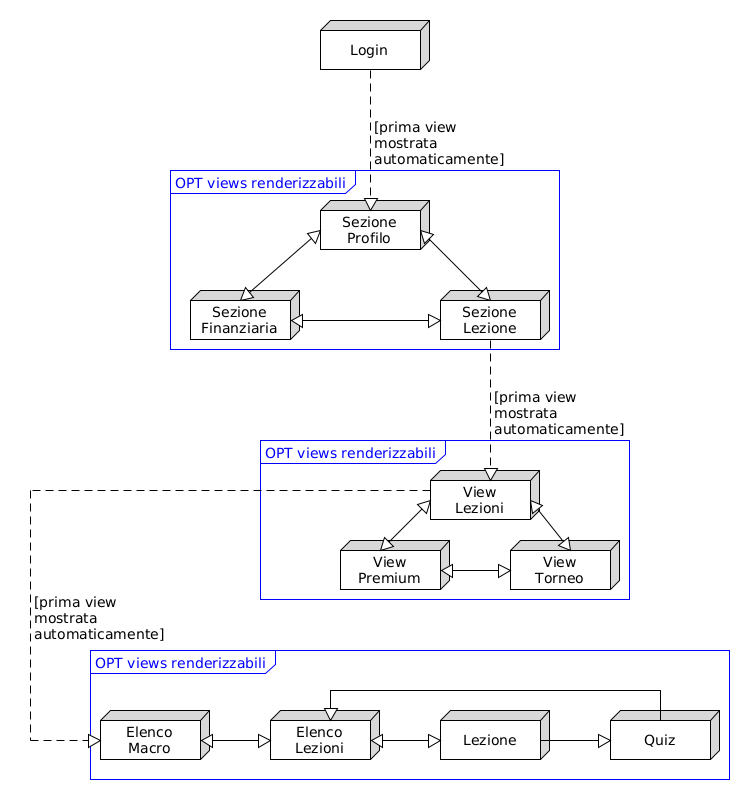
\includegraphics[scale=0.5]{pictures/schema_navigazione_schermate.png}}
    \hspace*{\dimexpr(\paperwidth-\textwidth)/15}
    \caption{Schema logico di navigazione delle schermate}
    \label{Schema logico di navigazione delle schermate}
\end{figure}



\begin{figure}[!htbp]
    \centering
    \makebox[0pt]{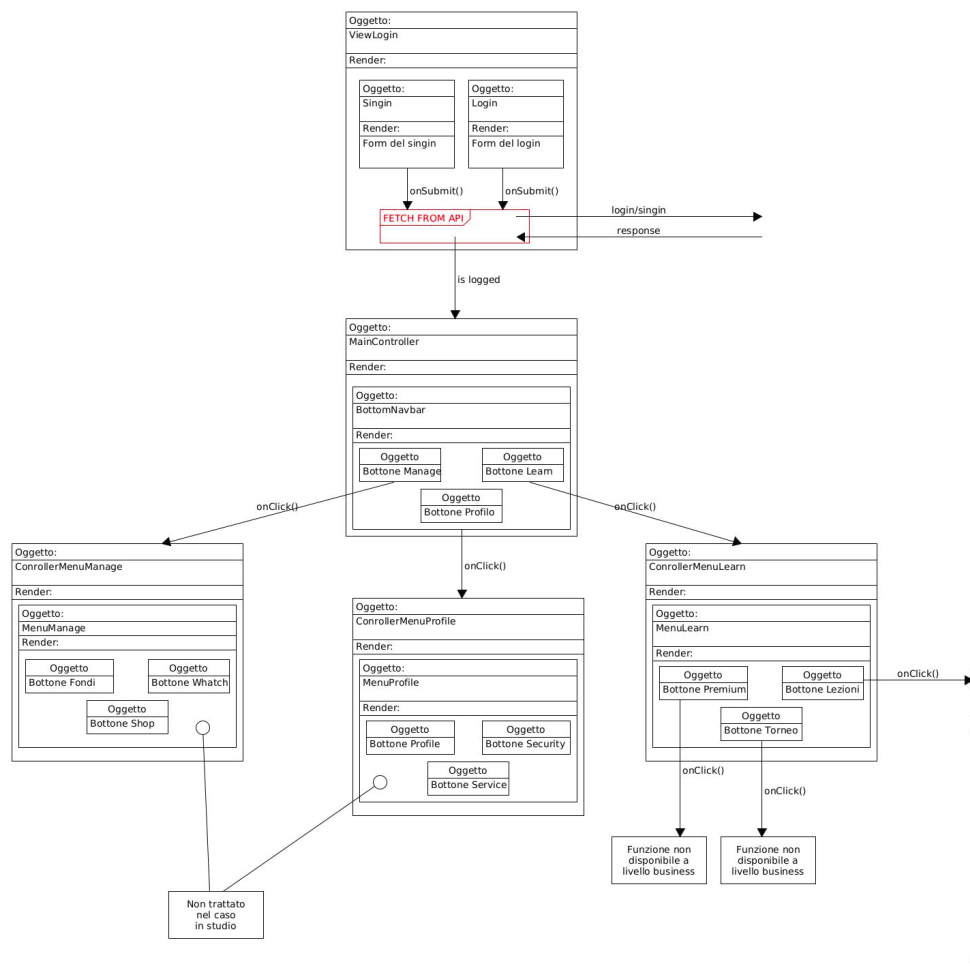
\includegraphics[scale=0.54, angle=270]{pictures/schema_generale_1.png}}
    \hspace*{\dimexpr(\paperwidth-\textwidth)/15}
    \caption{Schema della logica di funzionamento delle schermate pt.1}
    \label{Schema di funzionamento delle schermate pt.1}
\end{figure}


\begin{figure}[!htbp]
    \centering
    \makebox[0pt]{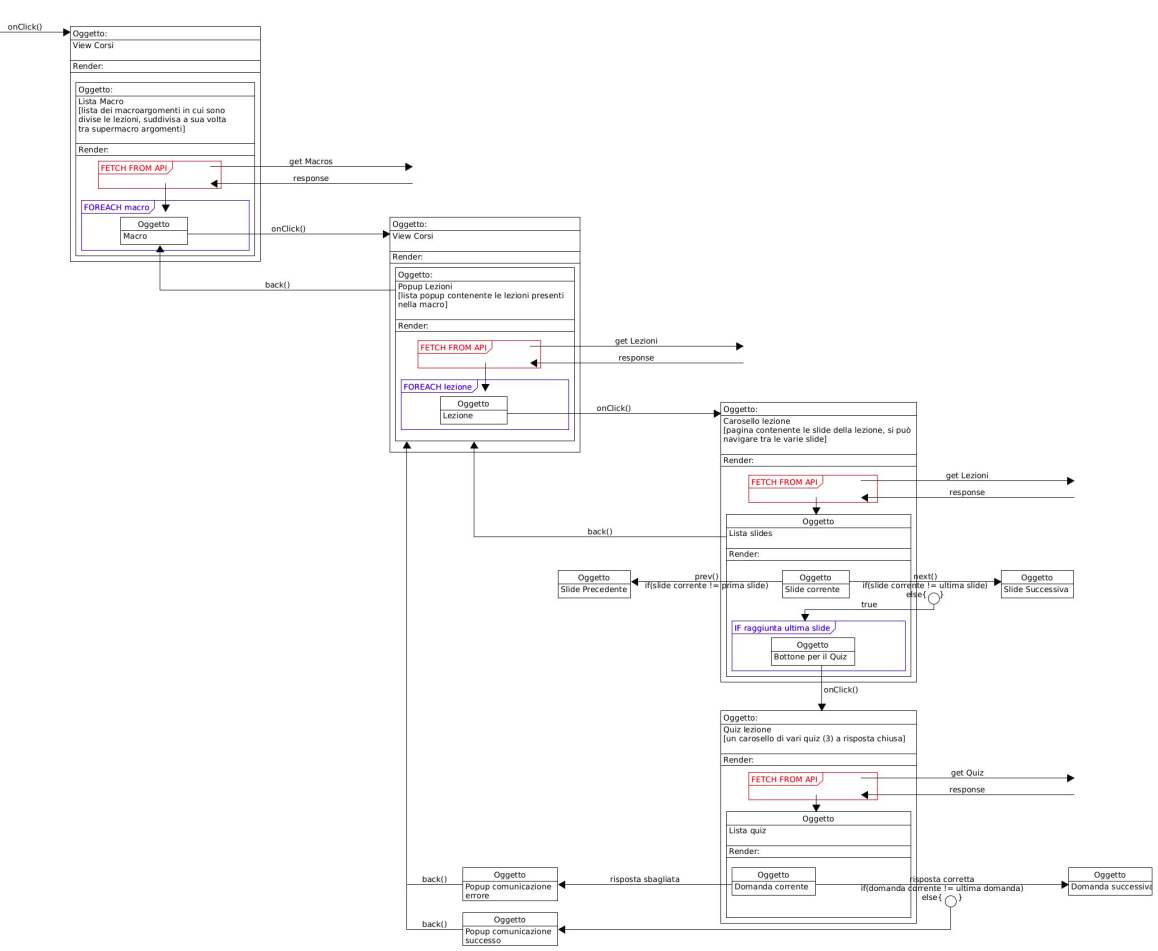
\includegraphics[scale=0.55, angle=270]{pictures/schema_generale_2.png}}
    \hspace*{\dimexpr(\paperwidth-\textwidth)/15}
    \caption{Schema della logica di funzionamento delle schermate pt.2}
    \label{Schema di funzionamento delle schermate pt.2}
\end{figure}






\newpage
\subsection{Backend}
Ho deciso di suddividere il backend in più api poiché essendo servizi piuttosto diversi tra loro voglio avere la possibilità di cambiare host, in base alla potenza o al livello di sicurezza che ritengo necessario per ogni singola api, senza dover aggiungere strati di complessità a quelle che non necessitano di particolare potenza o protezione.\\
L’api per recuperare i dati relativi alle lezioni deve semplicemente contattare un database e rispondere senza effettuare calcoli, non avrà quindi bisogno di particolare aumento di potenza di calcolo all’aumentare degli utenti. D’altra parte l’api per il calcolo del portafogli avrà bisogno di maggiore potenza all’aumentare degli utenti, poiché deve eseguire calcoli, e eventualmente essere posizionata sullo stesso server contenente un database di dati finanziari.\\
Altro caso in cui può essere necessaria una suddivisione potrebbe riguardare la sicurezza: le api per il calcolo dei portafogli e per recuperare le lezioni non hanno dei dati sensibili al loro interno, e se raggiunte o modificate da utenti malevoli il danno maggiore potrebbe essere l’utilizzo delle librerie o l’appropriarsi dei dati riguardanti le lezioni, cose tra l’altro disponibili gratuitamente con il download dell’app, quindi il danno più grave per il business potrebbe essere il blocco del loro corretto funzionamento.\\
Invece l’api da contattare per effettuare il login potrebbe esporre i dati sensibili e le credenziali di accesso degli utenti, che costituiscono una parte sensibile e di interesse per utenti malevoli, di conseguenza il livello di protezione dev’essere alto. Si può scegliere così di hostare l’api con i dati necessari al login su un server più sicuro, con un livello di crittografia maggiore e più protetto, cosa non necessaria per le api che recuperano esclusivamente dati non relativi all’utente, evitando così di aggiungere livelli di complessità non necessari che andrebbero a rallentarne il funzionamento.\\

\noindent
Confrontando le varie tecnologie disponibili ho selezionato Node.js per le api di login, lezioni e recupero dei dati finanziari principalmente per il suo funzionamento.\\
Node sfrutta l’interprete di javascript presente in Chrome, chiamato v8, che permette di risolvere le richieste in maniera non bloccante, tramite l’utilizzo di callback, migliorando la velocità del server. Ho utilizzato poi il framework Express per costruire un server con Node.\\
Invece per l’api per il calcolo dei portafogli ho preferito un server Python implementato tramite il microframework Flask. Questo framework leggero aggiunge solo gli elementi essenziali, evitando di dover riscrivere tanto codice “adapter” tra il server e l’utilizzo delle librerie. Per le librerie di calcolo dei portafogli ho scelto Python poiché permette uno sviluppo facile e veloce e ha molte librerie di calcolo complesso come “scipy” o “numpy” che evitano la riscrittura di complesse funzioni matematiche. Tuttavia Python non è particolarmente veloce e efficiente, perciò ho considerato l’opzione di dover riscrivere le librerie e l’api in un altro linguaggio per permettere una maggiore velocità dei calcoli.\\

\noindent
Il funzionamento generale delle API è molto simile, in generale il client invia una richiesta al server sull'ip pubblico con un certo path. Questa richiesta viene presa dal server web che la inoltra sulla porta corretta in base alla prima parte del path. Una volta arrivata all'api corretta il router, grazie alla seconda parte del path, richiama la funzione corrispondente. Questa funzione esegue i calcoli necessari, richiamando altre funzioni di libreria scritte da me, ne recupera il risultato e lo inoltra come risposta. In caso di errore invia un messaggio di errore di default.\\
La funzione richiamata dal router esegue delle operazioni preliminari prima di richiamare la funzione di libreria necessaria. Innanzitutto verifica che il database sia raggiungibile, se lo è richiama una funzione di login, per verificare che l'utente abbia i permessi per eseguire le operazioni. Se il login fallisce viene inviata una risposta al client che disconette l'utente, l'idea è che l'utente abbia una chiave per eseguire le operazioni, se questa chiave scade non può più eseguire operazioni, questo aumenta il livello di sicurezza poichè anche se viene intercettata una richiesta e decriptata, la chiave avrà solo un certo tempo per essere utilizzata. Se il login ha successo viene richiamata una funzione contenente le operazioni da eseguire e, una volta eseguite, viene inviata la risposta contenente i dati o l'esito positivo dell'operazione.

\subsubsection{Lista delle API}
Di seguito una lista con tutte le API e una loro breve descrizione.

\begin{enumerate}

\item[-] API di login    \begin{enumerate}
                            \item[-] \textbf{Linguaggio}: Node.js, Express
                            \item[-] \textbf{Richieste}: HTTP/POST
                            \item[-] \textbf{Descrizione}: API per effettuare login, singin e che gestisce il salvataggio e recupero dei dati personali relativi all'utente
                        \end{enumerate}
\item[-] API di finanza \begin{enumerate}
                            \item[-] \textbf{Linguaggio}:Node.js, Express
                            \item[-] \textbf{Richieste}: HTTP/POST
                            \item[-] \textbf{Descrizione}: API per effettuare tutte le operazioni riguardanti il lato finanziario quidni sia la gestione delle watchlists dell'utente, sia la gestione (acquisto o vendita) deli suoi portafogli
                        \end{enumerate}
\item[-] API delle lezioni \begin{enumerate}
                            \item[-] \textbf{Linguaggio}: Node.js, Express
                            \item[-] \textbf{Richieste}: HTTP/POST
                            \item[-] \textbf{Descrizione}: API che recupera i dati relativi alle lezioni e salva i progressi dell'utente
                        \end{enumerate}
\item[-] API del calcolatore \begin{enumerate}
                            \item[-] \textbf{Linguaggio}: Python, Flask
                            \item[-] \textbf{Richieste}: HTTP/POST
                            \item[-] \textbf{Descrizione}: API che calcola il portafoglio di ottimo in base al tipo di portafoglio richiesto e ai dati inviati
                        \end{enumerate}

\end{enumerate}


\newpage
\begin{figure}[!ht]
    \centering
    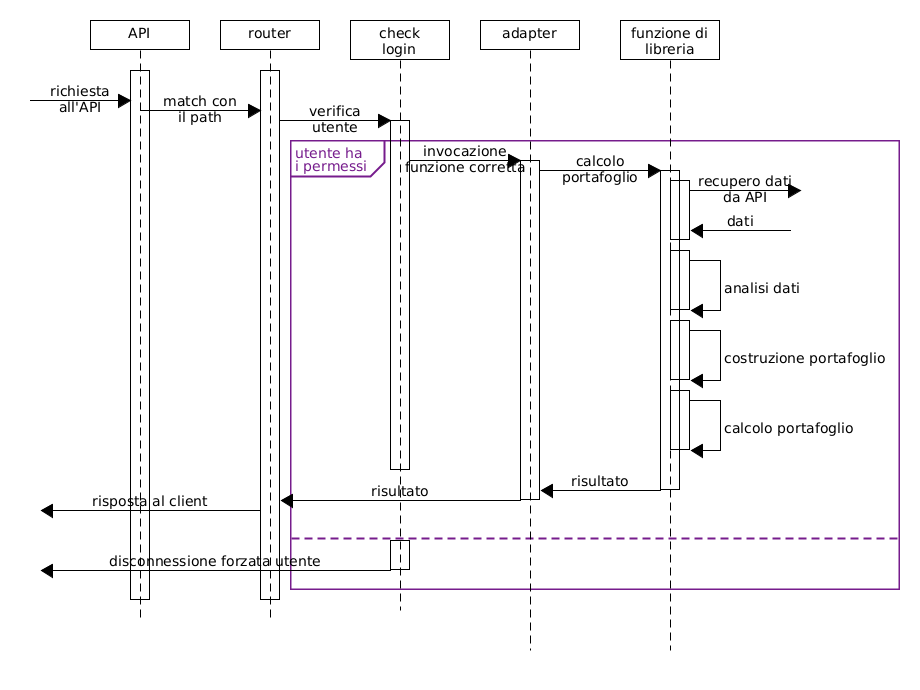
\includegraphics[scale=0.6, angle=270]{pictures/schema_generale_api_python.png}
    \caption{Schema di logica generale del funzionamento dell'API scritta in Python}
    \label{DSD dell'API Python}
\end{figure}

\begin{figure}[!ht]
    \centering
    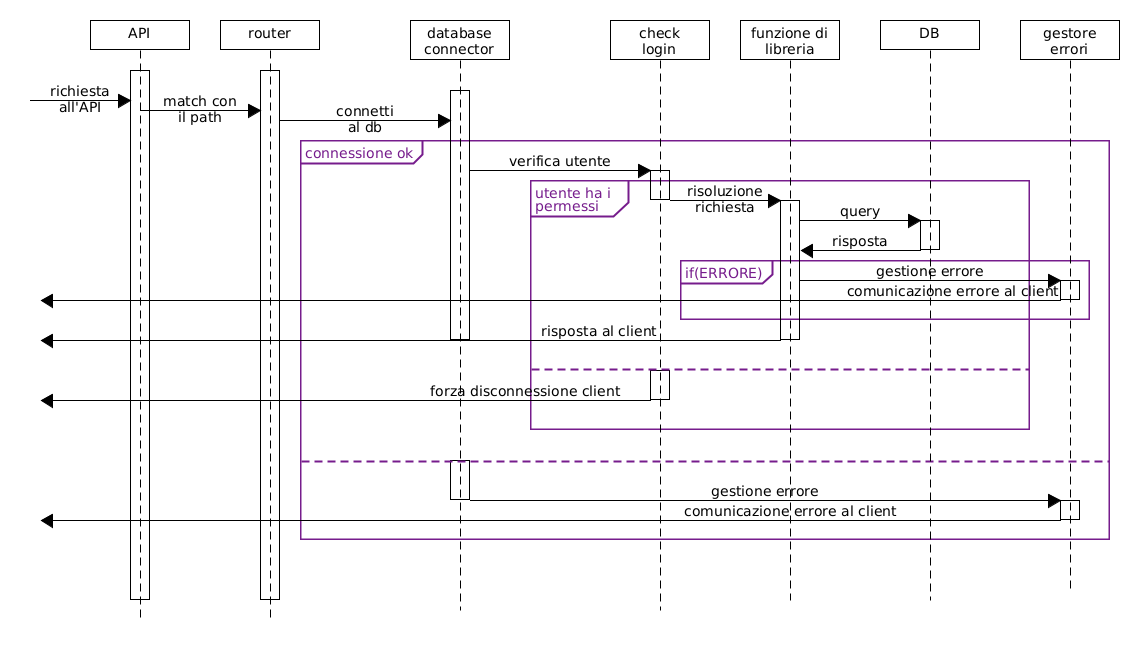
\includegraphics[scale=0.6, angle=270]{pictures/schema_generale_api_node.png}
    \caption{Schema di logica generale del funzionamento di un'API scritta in Node}
    \label{DSD delle API Node}
\end{figure}
